\documentclass[11pt]{article}
\usepackage[utf8]{inputenc}
\usepackage[english]{babel}
\usepackage{amsmath}
\usepackage{graphicx}
\usepackage{float}
\usepackage{lipsum}
\usepackage{multicol}
\usepackage{xcolor}
\usepackage{tabularx}
\usepackage{booktabs}
\usepackage{hyperref}
\newcolumntype{Y}{>{\centering\arraybackslash}X}
\usepackage[left=2.00cm, right=2.00cm, top=2.00cm, bottom=2.00cm]{geometry}

\title{AN2DL Reports Template}

\begin{document}
    
    \begin{figure}[H]
        \raggedright
        
\includegraphics[scale=0.5]{polimi.png} \hfill 
\includegraphics[scale=0.3]{airlab.jpeg}
    \end{figure}
    
    \vspace{5mm}
    
    \begin{center}
        {\Large \textbf{AN2DL - First Challenge Report}}\\
        \vspace{2mm}
        {\Large \textbf{theoverfitters}}\\
        \vspace{2mm}
        {\large Raul Agolli,}
        {\large Kevin Pio Abate,}
        {\large Andrea Ascenzo Mastroberti}\\
        \vspace{2mm}
        {\large raulagolli,}
        {\large keevin16,}
        {\large drebishh}\\
        \vspace{5mm}
        November 2025
    \end{center}    
    \vspace{5mm}
    
    \begin{multicols}{2}
        
        \section{Introduction}
        The goal of this challenge is to determine each subject’s true pain status from multivariate time series data. The dataset, \textit{The Pirate Pain Dataset}, captures temporal patterns of body joints and pain perception from both ordinary individuals and pirates. The target classes are \textbf{no\_pain}, \textbf{low\_pain}, and \textbf{high\_pain}.\\
 
        \begin{figure}[H]
    \centering
    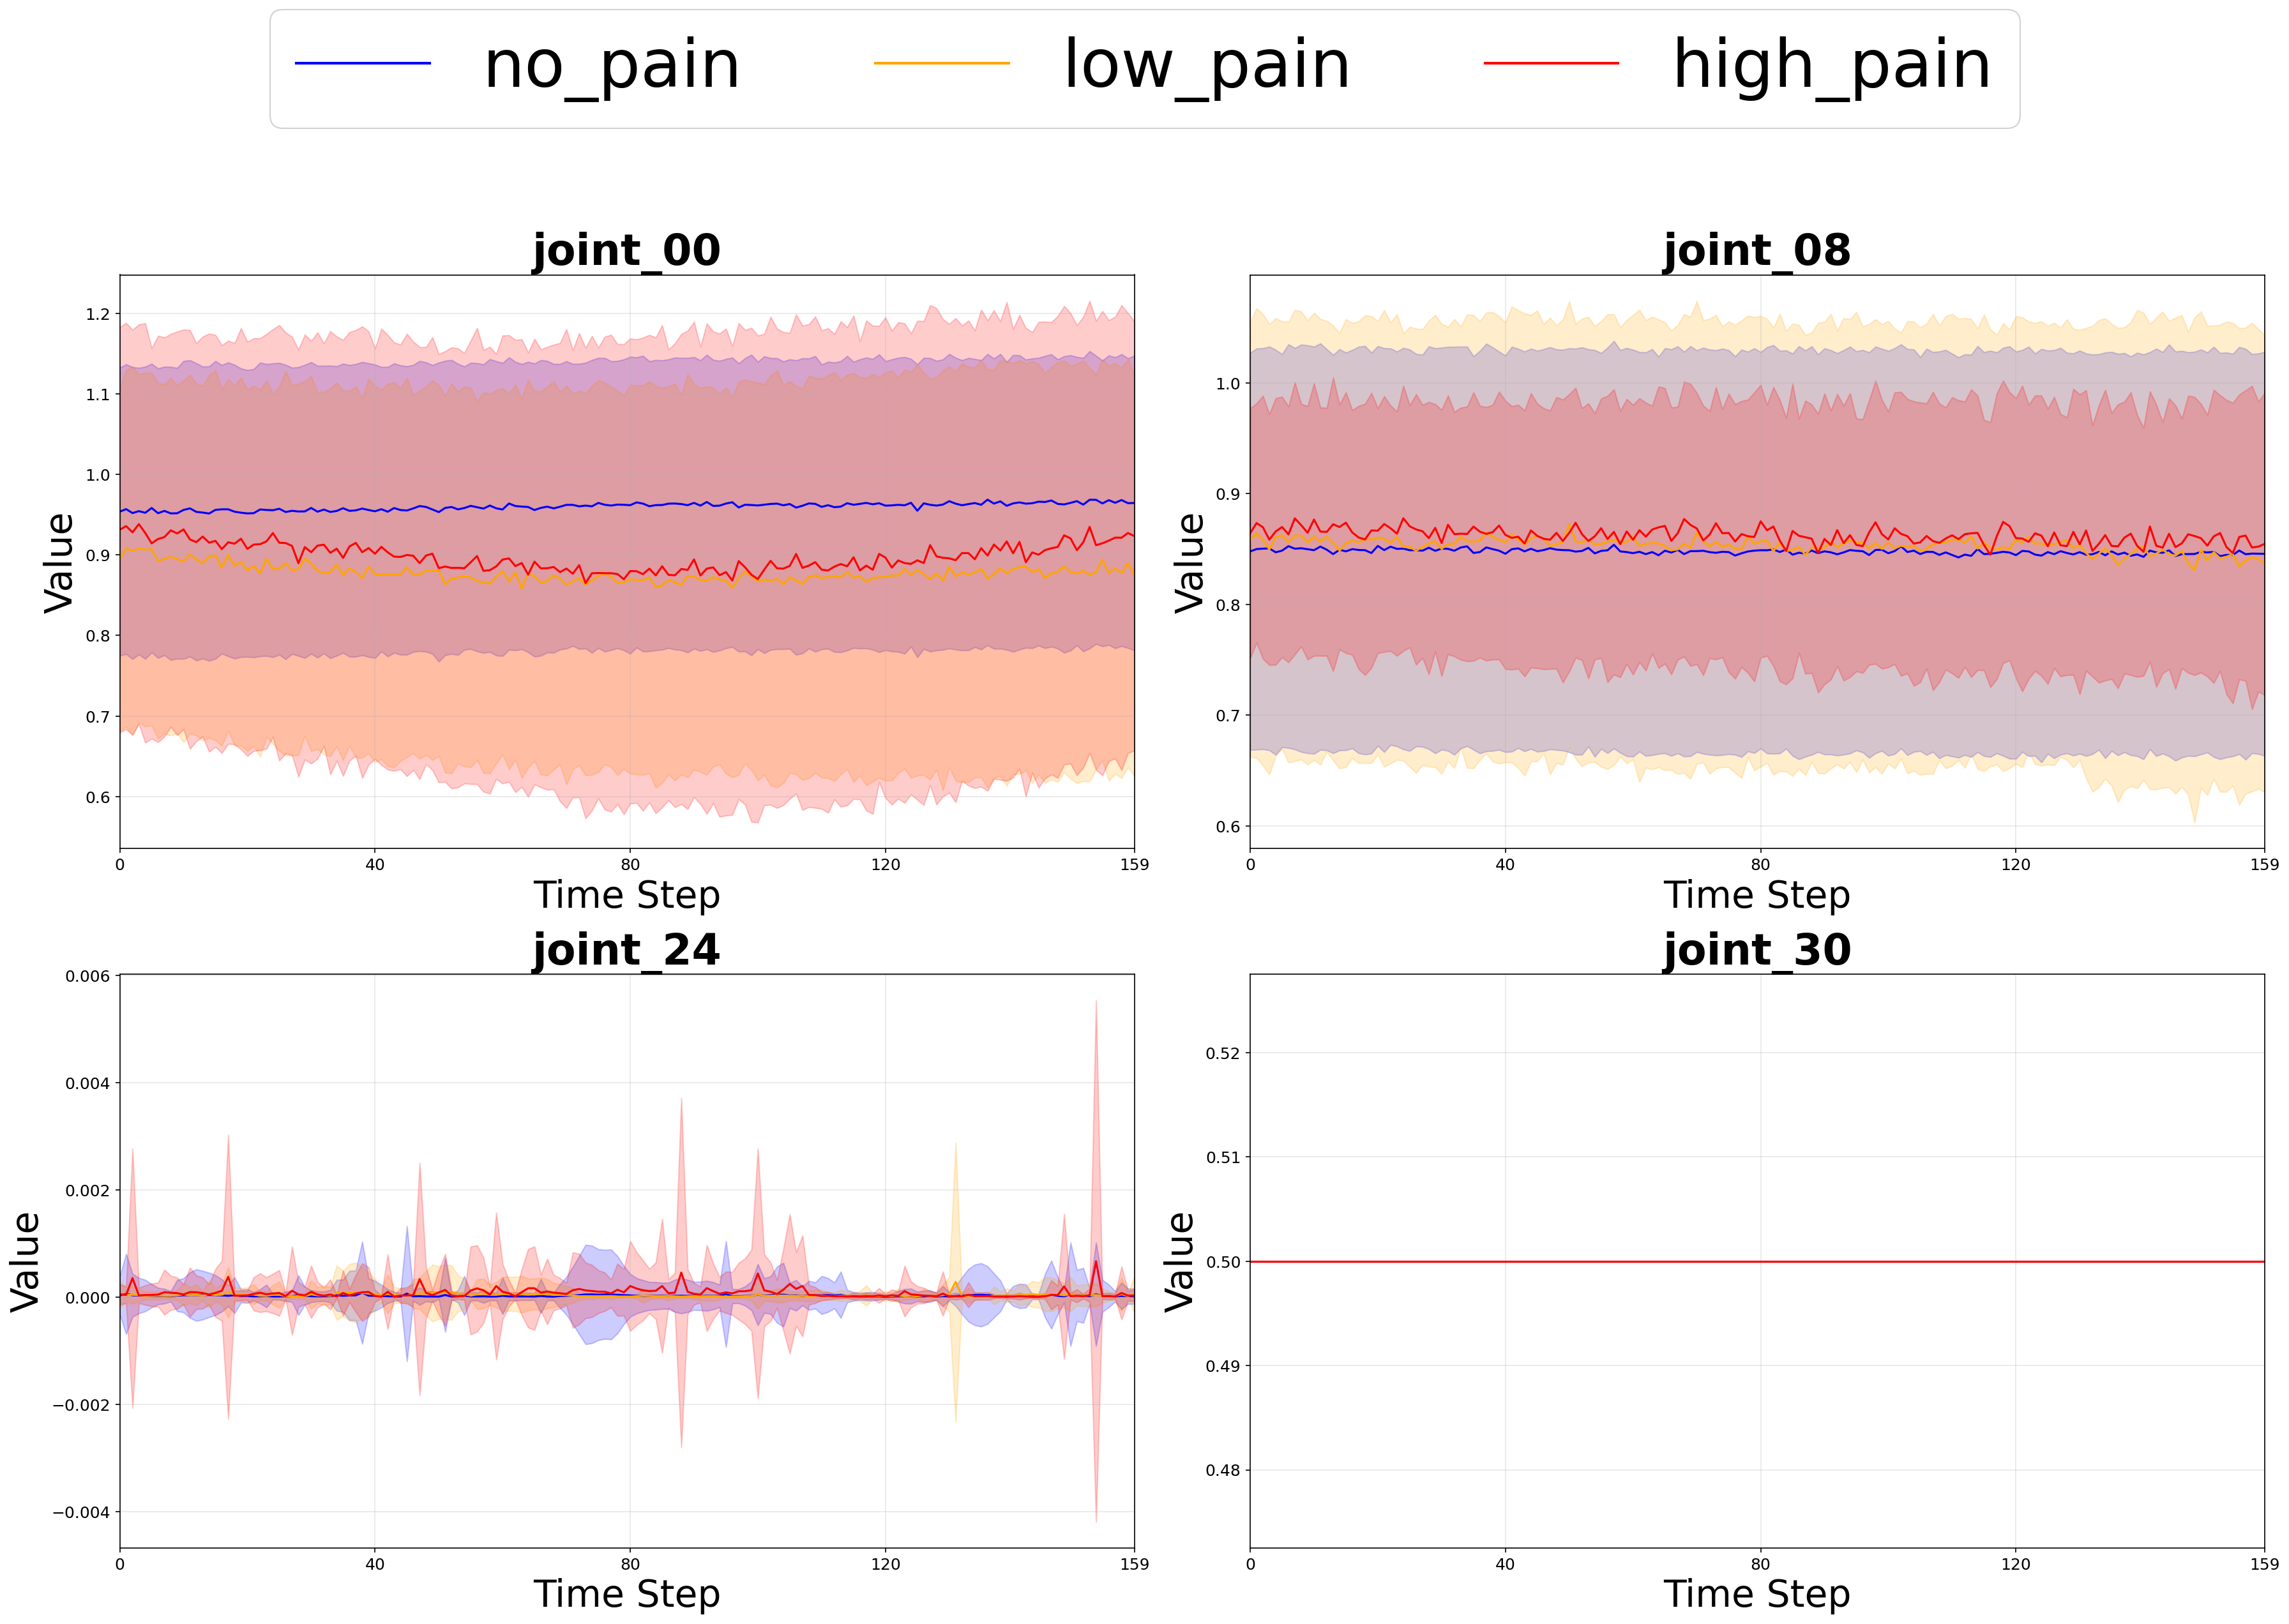
\includegraphics[
        width=0.4\textwidth,
        keepaspectratio
    ]{images/only4.png}
    \caption{Mean and standard deviation by pain class of some joint features}
\end{figure}
    
        %\noindent We progressively moved from a simple RNN baseline to more advanced architectures, exploring convolutional layers, attention mechanisms, an ensemble setup and ultimately an hybrid dual-model strategy (one network performs Pain vs.\ No Pain detection, while a second distinguishes Low vs.\ High Pain, and their outputs are merged through a soft-cascade ensemble).
        
        \section{Problem Analysis}
        The dataset presents several challenges inherent to time-series classification, our initial focus was on analyzing available techniques to address them effectively.
        \subsection{Challenges}
        The main challenges of this study are the \textbf{limited size} of the dataset and its \textbf{imbalance}.\\
        The dataset contains only 660 pirates' samples with 160 timesteps and 40 features, creating a high-dimensional setting where larger models are prone to overfitting. To address this, we performed several preprocessing steps.
        \begin{itemize}
            \item \textbf{Pain survey consolidation}:
            The four pain-assessment series were merged into a single integer feature by taking the median and flooring the result. The original columns were removed.
        \end{itemize}
        \begin{itemize}
            \item \textbf{Morphological feature merging:} The categorical features \texttt{n\_legs}, \texttt{n\_hands}, and \texttt{n\_eyes} were compressed into a binary flag (\texttt{pirate}), set to 0 for normal subjects and 1 for malformed ones.
        \end{itemize}
        \begin{itemize}
            \item \textbf{Constant feature removal:} The feature \texttt{joint\_30}, which had a constant value of 0.5 across all samples, was dropped.
        \end{itemize}
        \begin{itemize}
            \item \textbf{2D Sinusoidal Positional Encoding: }     
            To facilitate the model's recognition of cyclical dependencies and avoid linear time index boundary effects, a 2D sinusoidal positional encoding (PE) was implemented. Utilizing a {\textbf{PERIOD}} = 80, the original $\mathbf{time}$ feature was replaced by two continuous variables:

            $$\mathbf{time\_sin} = \sin \left(\frac{2 \pi \cdot time}{80}\right)$$
            $$\mathbf{time\_cos} = \cos \left(\frac{2 \pi \cdot time}{80}\right)$$This embedding maps time onto a unit circle, explicitly modeling temporal proximity across the period boundary.
        \end{itemize}
        \begin{itemize}
            \item \textbf{Scaling}: Continuous features were scaled using \textit{MinMax Scaling}. To handle varying sequence lengths and augment the data, we employed a sliding window approach with tunable window sizes and strides.
        \end{itemize}
        
        \section{Method}
        We began our experiments with a simple RNN model to establish a baseline for our approach. Our initial focus was on preprocessing and augmenting the dataset to improve model performance.
        \subsection{Data Augmentation}
        We experimented with various augmentation techniques, including Generative Adversarial Network (GAN), Gaussian noise and Time Warping. However, these methods did not yield any significant improvement in performance. Consequently, we decided to discontinue their use and to work on the original data.
        Our focus switched on other aspects of the pipeline.

        \subsection{Network Architecture Exploration}
        Given the limited success with the initial network, we decided to explore stronger models without altering the dataset further.
        We experimented the RNN with windowing, a \textbf{Dual-Model} strategy where we trained two specialized binary classifiers, M1 for classifying no pain vs. pain (combining low and high), and M2 Classifies low pain vs high pain (trained only on pain samples). However, these were too large and complex, often resulting in poor validation performance, likely due to overfitting.
        \\Afterward, we attempted to implement a custom network inspired by the CSHN\cite{CSHN}.
        \subsection{Implementation and Customization}
        %Furthermore, we enhanced the performance of our network by experimenting with various modules, testing them individually to track their differential impact on results.\\
       Our best-performing model consists of a three-layer 1D CNN, combining \textbf{convolutional} and \textbf{normalization} layers, followed by a\textbf{ Global Average Pooling} (GAP) layer to reduce the dimensionality of the feature maps before classification. This structure helps maintain a compact set of parameters and contributes to improved computational efficiency. The CNN output is then passed to a \textbf{Recurrent Neural Network} (LSTM) to capture temporal dependencies within the time series.\\ After that the \textbf{Attention Layer}: was employed to significantly enhance the network’s ability to focus on informative features by adaptively recalibrating the importance of inputs across the temporal sequence.\\\\
        %\noindent Our best-performing solution is a \textbf{single hybrid architecture} incorporating a 3-layer 1D CNN for feature extraction, a Recurrent Neural Network (LSTM), and a dedicated \textbf{static feature branch}. This branch explicitly models the \textbf{"pirate"} morphological characteristics, adding a learnable bias to the final classification logits. This unified approach achieved robust performance through a 10-Fold Cross-Validation scheme.
        %Our final solution relies on a e hybrid network (CSHN), in the proposed model we employ a Convolutional Neural Network (CNN) and Gated Recurrent Unit (GRU) network, harnessing the complementary strengths of both architectures.CNN excels in local feature learning while GRU demonstrates superior sequence feature learning capabilities.
        \subsection{Class Imbalance Resolution}
        A significant improvement was made when, analyzing the class distribution, we discovered that the low\_pain and high\_pain classes were too small for our classification scope. As a result, we adjusted the class weights to be inversely proportional to their frequencies. This adjustment led to a drastic improvement of the performance on both the validation and test datasets.
    \begin{figure}[H]
        \centering
     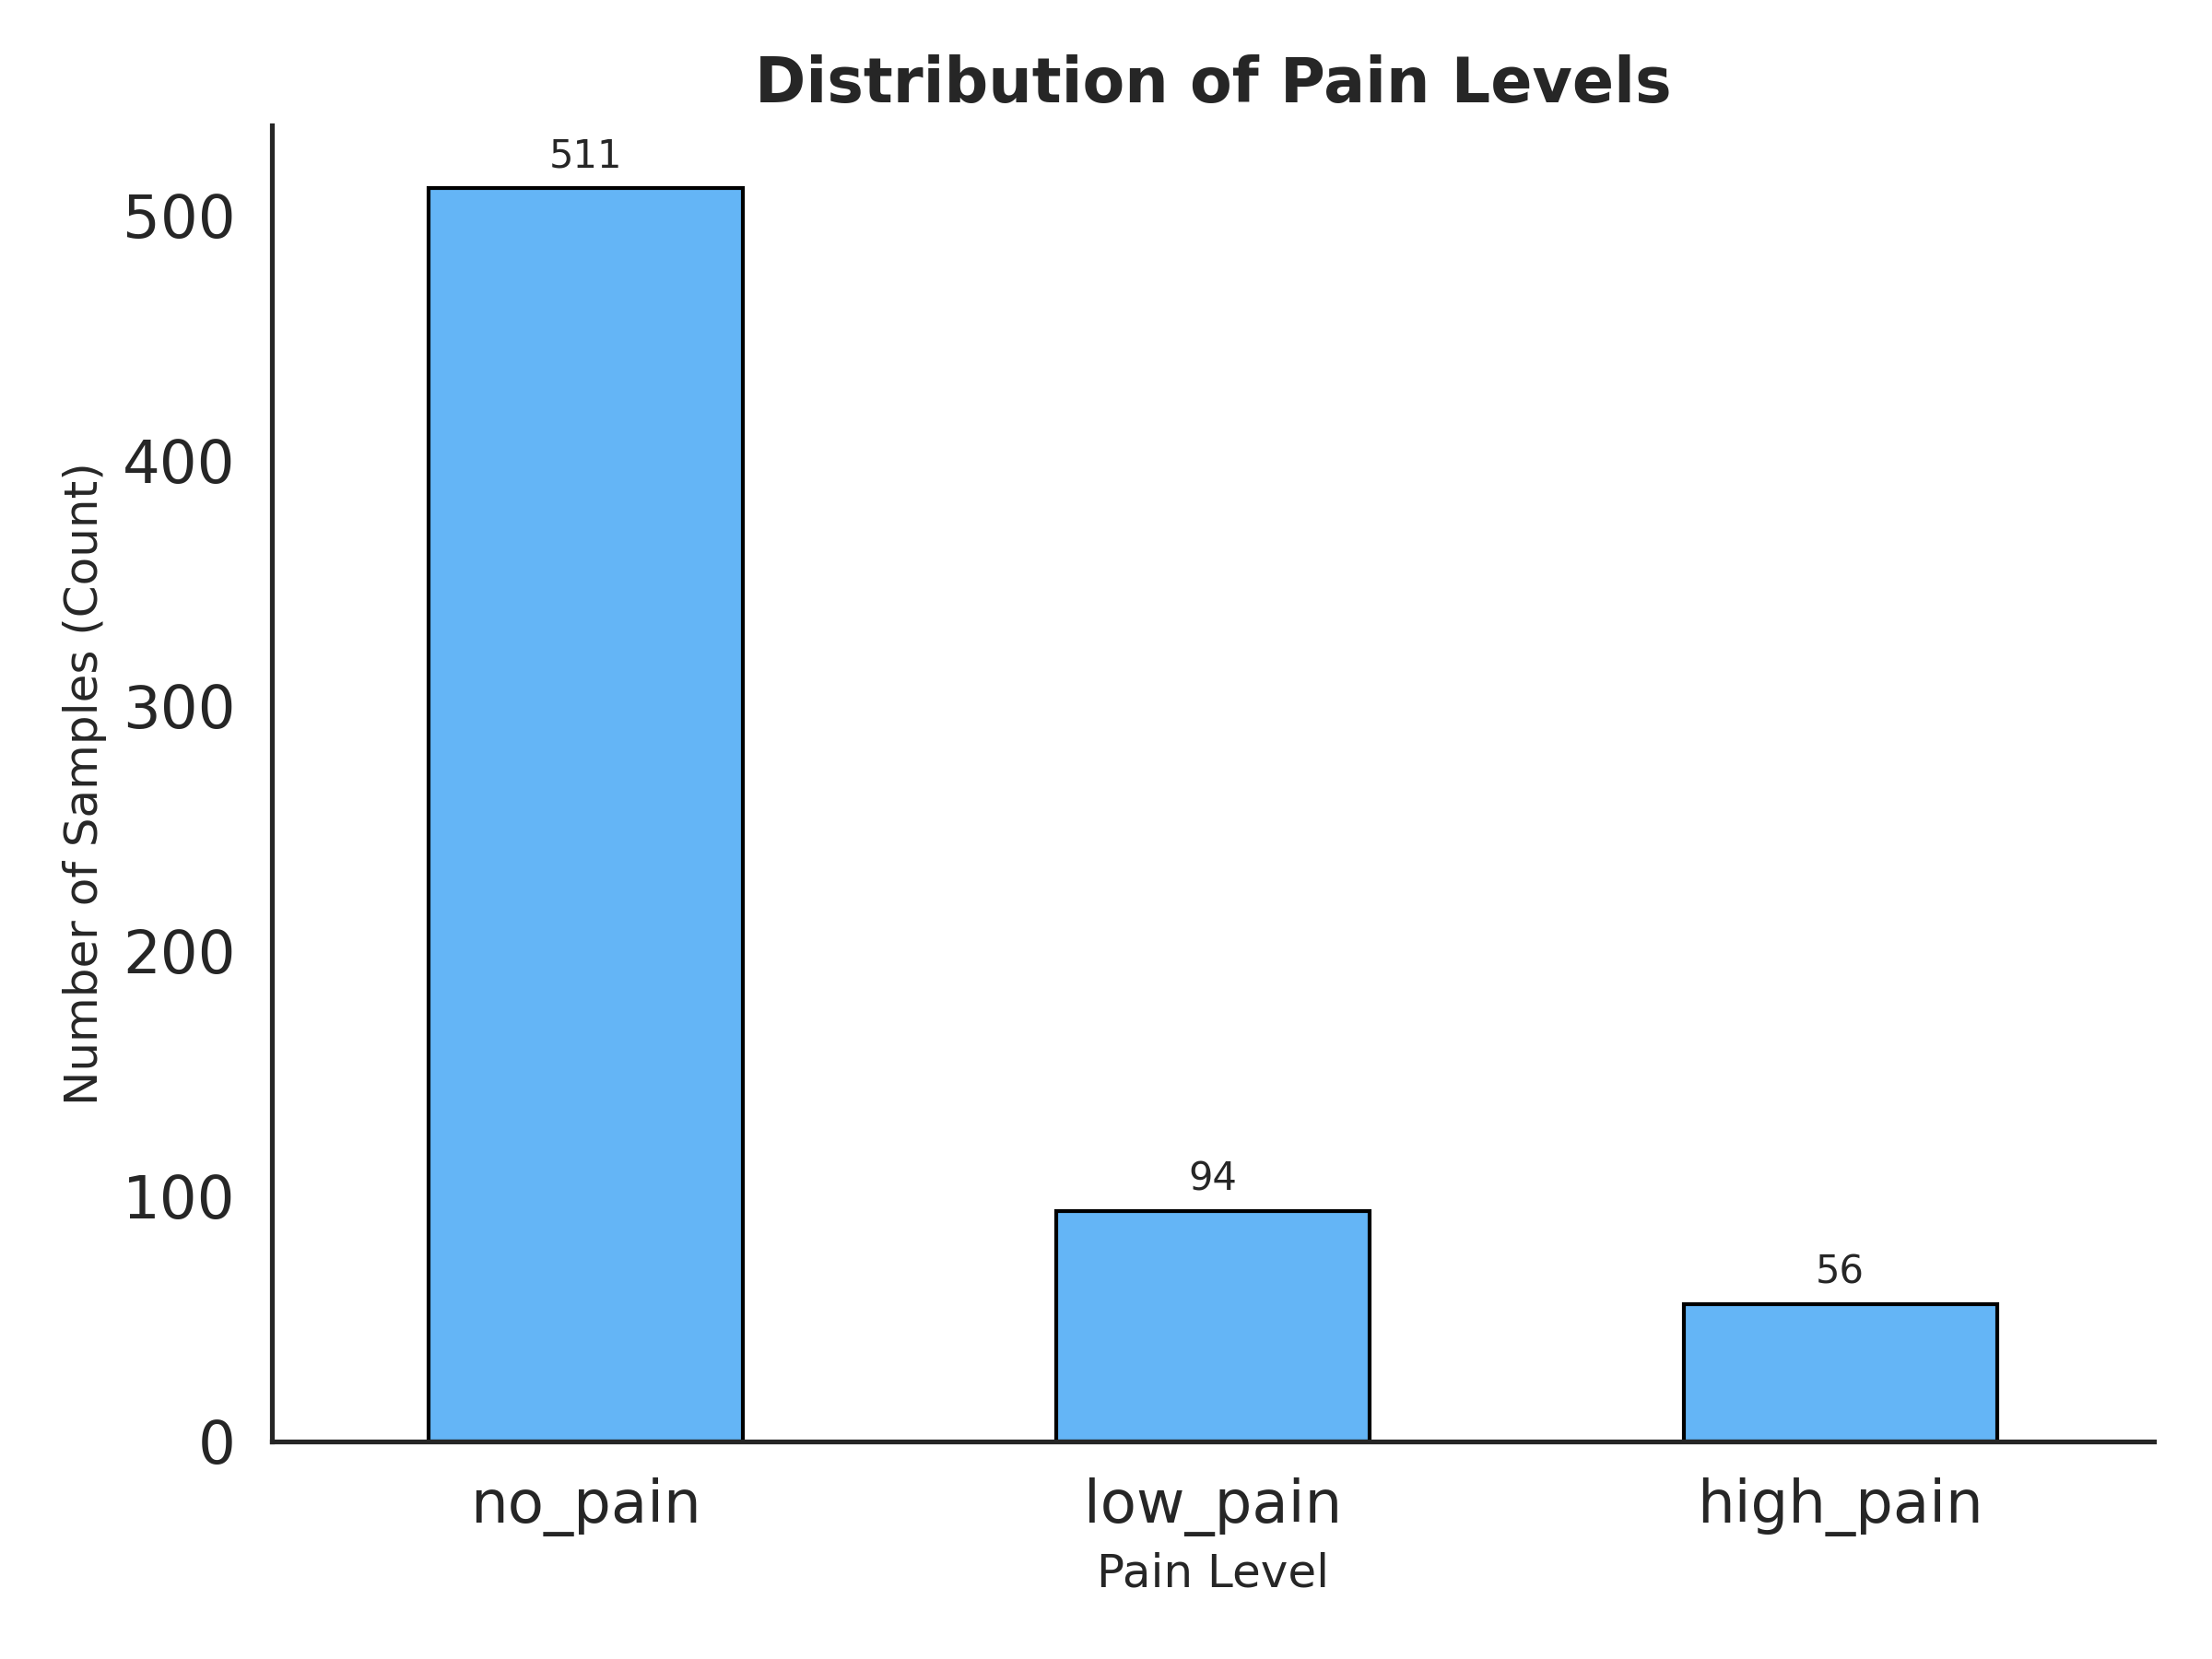
\includegraphics[
         width=0.5\textwidth,
         keepaspectratio
     ]{images/classImbalance.png}
        \caption{Distribution of the classes on the unbalanced dataset}
    \end{figure}  
        \subsection{Loss Function}
  We explored several loss functions and tuned their associated parameters to assess their effectiveness. Among the tested options, \textbf{weighted Cross-Entropy} provided the most reliable performance. In contrast, Focal Loss did not lead to measurable improvements, and the application of label smoothing consistently degraded results.\\ We attempted to solve frequent high-pain/no-pain misclassifications by applying a penalty to those mispredictions in the cross entropy as well, with mild improvements. %Overall, the only substantial and reproducible gains were achieved using Cross-Entropy with class weights, which effectively mitigated the impact of class imbalance.

   
        
        
        \section{Experiments}
        We used \textbf{PyTorch} for model implementation and \textbf{Optuna} for hyperparameter tuning.
        
        \subsection{Hyperparameter Tuning}
       We dedicated the majority of our training experiments to hyperparameter optimization, with Optuna, carefully assessing the impact of each adjustment in order to guide the model toward the desired performance.\\
        We assessed the model using 4-Fold Cross-Validation with fold-level multi-GPU parallelization and pruning to speed computation. \\The best parameters (Trial 71) were:\\
        \textbf{Window Size}: 20 time steps\\
        \textbf{Stride}: 5 time steps (high overlap for augmentation)\\
        \textbf{CNN Filters}: 8 $\to$ 16 $\to$ 32\\
        \textbf{RNN}: LSTM, 1 Layer, Hidden Size 8\\
        \textbf{Dropout}: CNN 0.26, RNN 0.59\\
        \textbf{Optimizer}: AdamW with $lr=3.5e^{-4}$ and weight decay $2.2e^{-5}$\\
    
        
        \subsection{Training Protocol}
        To ensure robustness, the best configuration was retrained using \textbf{Stratified Group 10-Fold Cross-Validation}. This prevents data leakage by ensuring all windows from the same subject remain in the same fold. We used Standard Cross Entropy Loss (weighted) and Early Stopping.
        
        \section{Results}
        The model demonstrated high stability across the 10 folds. The aggregated validation results are presented below.
        
        \begin{table}[H]
            \centering
            \caption{10-Fold CV Aggregated Metrics (Best Epoch)}
            \begin{tabularx}{\linewidth}{lY}
                \toprule
                Metric & Value \\
                \midrule
                Accuracy & 0.9218 \\
                F1-Score (Macro) & 0.8316 \\
                \textbf{F1-Score (Weighted)} & \textbf{0.9207} \\
                \bottomrule
            \end{tabularx}
            \label{tab:Performance}
        \end{table}
        
        \section{Discussion}
        The success of the single hybrid model over the dual-model ensemble suggests that the feature space is most likely better learned jointly. The sliding window with a small stride (5) was crucial, significantly increasing the effective training set size and allowing the small LSTM (hidden size 8) to generalize well without overfitting. The static branch provided a necessary bias correction for the "pirate" subjects, who likely exhibit different movement baselines.
        
        \section{Conclusions}
        We successfully developed a robust pipeline for pain classification using a Hybrid CNN-LSTM architecture with a static feature branch. The key contributions were the explicit modeling of morphological data and the aggressive windowing strategy tuned via Optuna. The final model achieves a weighted F1-score of \textbf{0.92} in cross-validation.
        
        % \bibliography{references}
        % \bibliographystyle{abbrv}
        \begin{thebibliography}{9}
        
        \bibitem{CSHN}
    Wang, X., Zhang, Y., Bai, N., Yu, Q., \& Wang, Q. (2024). Class-imbalanced time series anomaly detection method based on cost-sensitive hybrid network. \textit{Expert Systems With Applications}, 238, 122192.

\end{thebibliography}

    \end{multicols}
\end{document}